\documentclass[letter,11pt]{article}

\usepackage[spanish,es-nodecimaldot]{babel}
\usepackage[utf8]{inputenc}

\usepackage{lmodern}
\usepackage[T1]{fontenc}
\usepackage{textcomp}

\usepackage{framed}
\usepackage[svgnames]{xcolor}
\colorlet{shadecolor}{Gainsboro!50}

\usepackage[labelfont=bf]{caption}
\usepackage{graphicx}
\usepackage{pstricks}

\usepackage{anysize}
\marginsize{3cm}{2cm}{2cm}{3cm}

\usepackage{siunitx}
\usepackage{amsmath}
\usepackage{array}
\usepackage{csquotes}
\usepackage{steinmetz}

\usepackage{fancyhdr}
\usepackage{lastpage}
\pagestyle{fancy}
\fancyhf{}
\fancyhead[LE,RO]{Laboratorio de Circuitos Eléctricos III}
\fancyfoot[CO,CE]{\thepage\ de \pageref{LastPage}}

\special{papersize=215.9mm,279.4mm}

\usepackage[
    pdfauthor={Carlos Eduardo Caballero Burgoa},%
    pdftitle={Laboratorio de Circuitos Eléctricos III},%
    pdfsubject={Circuitos trifásicos desequilibrados con fuente delta y carga
    delta},%
    colorlinks,%
    citecolor=black,%
    filecolor=black,%
    linkcolor=black,%
    urlcolor=black,
    breaklinks]{hyperref}
\usepackage{breakurl}

\renewcommand{\arraystretch}{1.2}

\begin{document}

\begin{titlepage}
    \begin{center}
        {\Large UNIVERSIDAD MAYOR DE SAN SIMÓN}\\
        \vspace*{0.15cm}
        {\large FACULTAD DE CIENCIAS Y TECNOLOGÍA}\\
        \vspace*{0.10cm}
        DEPARTAMENTO DE ELÉCTRICA-ELECTRÓNICA\\
        \vspace*{3.0cm}
        {\Large \textbf{LABORATORIO DE CIRCUITOS ELÉCTRICOS III}}\\
        \vspace*{0.3cm}
        {\Large \textbf{INFORME No. 4}}\\
        \vspace*{3.5cm}
        {\Large \textbf{CIRCUITOS TRIFÁSICOS DESEQUILIBRADOS \\
        CON FUENTE DELTA Y CARGA DELTA}}\\
    \end{center}

    \vspace*{5.8cm}
    \leftskip=7.95cm
    \noindent
    \textbf{Estudiante:}\\
    Caballero Burgoa, Carlos Eduardo.\\
    \newline
    \textbf{Carrera:}\\
    Ing. Electromecánica.\\
    \newline
    \textbf{Docente:}\\
    Ing. Marco Antonio Vallejo Camacho.\\
    \newline
    \textbf{Grupo:} 2F (Martes).\\
\textbf{Fecha de entrega:} 15 de Octubre del 2024.\\
\end{titlepage}

\section{Cálculos teóricos}
Considerando un circuito trifásico delta-delta desequilibrado
(\textbf{Figura~\ref{circuito1}}) con las siguientes cargas:

\begin{itemize}
    \item \textbf{Carga A}: $R_1=1[k\Omega]$.
    \item \textbf{Carga B}: $R_2=250[\Omega]$ y $L=1[H]$.
    \item \textbf{Carga C}: $R_3=500[\Omega]$ y $C=10[\mu F]$.
\end{itemize}

Con voltajes de linea $U_L=220[\text{V}]$ y con frecuencia de $50[\text{Hz}]$,
se hallan las corrientes de fase y linea para los siguientes casos:

\begin{figure}[!h]
\centering
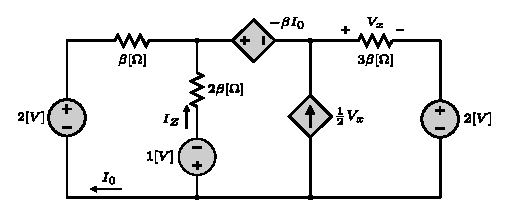
\includegraphics[scale=1.00]{figura1.eps}
\caption{Circuito trifásico desequilibrado delta-delta.}
\label{circuito1}
\end{figure}

\subsection{Secuencia positiva}
Se calcula la frecuencia angular ($\omega$):
\begin{equation*}
    \begin{split}
        \omega &= 2\pi f\\
               &= 2\pi(50)\\
               &= 100\pi[\text{rad}/\text{s}]\\
    \end{split}
\end{equation*}

Se hallan las impedancias en el dominio de frecuencia:
\begin{equation*}
    \begin{split}
        Z_1 &= R_1\\
            &= 1000[\Omega]\\
    \end{split}
\end{equation*}

\begin{equation*}
    \begin{split}
        Z_2 &= R_2+j\omega L\\
            &= 250+j100\pi[\Omega]\\
    \end{split}
\end{equation*}

\begin{equation*}
    \begin{split}
        Z_3 &= R_3+\frac{1}{j\omega C}\\
            &= 500-j\frac{1000}{\pi}[\Omega]\\
    \end{split}
\end{equation*}

Considerando una secuencia positiva:
\begin{equation*}
    \begin{split}
        \bar{U}_{L_1L_2} = 220\phase{0^{\circ}}\,[\text{V}]\\
        \bar{U}_{L_2L_3} = 220\phase{-120^{\circ}}\,[\text{V}]\\
        \bar{U}_{L_3L_1} = 220\phase{120^{\circ}}\,[\text{V}]\\
    \end{split}
\end{equation*}

A partir de los voltajes de linea, se calculan las corrientes de fase:
\begin{equation*}
    \begin{split}
        \bar{I}_{Z_1} &= \frac{\bar{U}_{L_1L_2}}{Z_1}\\
                      &= \frac{220\phase{0^{\circ}}}{500}\\
                      &= 0.22\phase{0^{\circ}}[\text{A}]\\
    \end{split}
\end{equation*}
\begin{equation*}
    \begin{split}
        \bar{I}_{Z_2} &= \frac{\bar{U}_{L_2L_3}}{Z_2}\\
                      &= \frac{220\phase{-120^{\circ}}}{500+j100\pi}\\
                      &= 0.55\phase{-171.49^{\circ}}[\text{A}]\\
    \end{split}
\end{equation*}
\begin{equation*}
    \begin{split}
        \bar{I}_{Z_3} &= \frac{\bar{U}_{L_3L_1}}{Z_3}\\
                      &= \frac{220\phase{120^{\circ}}}{500-j(1000/\pi)}\\
                      &= 0.37\phase{152.48^{\circ}}[\text{A}]\\
    \end{split}
\end{equation*}

Con las corrientes de fase se calculan las corrientes de linea:
\begin{equation*}
    \begin{split}
        \bar{I}_{L_1} &= \bar{I}_{Z_1}-\bar{I}_{Z_3}\\
                      &= 0.22\phase{0^{\circ}}-0.37\phase{152.48^{\circ}}\\
                      &= 0.58\phase{-17.34^{\circ}}[\text{A}]\\
    \end{split}
\end{equation*}
\begin{equation*}
    \begin{split}
        \bar{I}_{L_2} &= \bar{I}_{Z_2}-\bar{I}_{Z_1}\\
                      &= 0.55\phase{-171.49^{\circ}}-0.22\phase{0^{\circ}}\\
                      &= 0.77\phase{-173.92^{\circ}}[\text{A}]\\
    \end{split}
\end{equation*}
\begin{equation*}
    \begin{split}
        \bar{I}_{L_3} &= \bar{I}_{Z_3}-\bar{I}_{Z_2}\\
                      &= 0.37\phase{152.48^{\circ}}-
                         0.55\phase{-171.49^{\circ}}\\
                      &= 0.33\phase{49.89^{\circ}}[\text{A}]\\
    \end{split}
\end{equation*}

\subsection{Secuencia negativa}
Considerando una secuencia negativa:
\begin{equation*}
    \begin{split}
        \bar{U}_{L_1L_2} = 220\phase{0^{\circ}}\,[\text{V}]\\
        \bar{U}_{L_2L_3} = 220\phase{120^{\circ}}\,[\text{V}]\\
        \bar{U}_{L_3L_1} = 220\phase{-120^{\circ}}\,[\text{V}]\\
    \end{split}
\end{equation*}

A partir de los voltajes de linea, se calculan las corrientes de fase:
\begin{equation*}
    \begin{split}
        \bar{I}_{Z_1} &= \frac{\bar{U}_{L_1L_2}}{Z_1}\\
                      &= \frac{220\phase{0^{\circ}}}{500}\\
                      &= 0.22\phase{0^{\circ}}[\text{A}]\\
    \end{split}
\end{equation*}
\begin{equation*}
    \begin{split}
        \bar{I}_{Z_2} &= \frac{\bar{U}_{L_2L_3}}{Z_2}\\
                      &= \frac{220\phase{120^{\circ}}}{500+j100\pi}\\
                      &= 0.55\phase{68.51^{\circ}}[\text{A}]\\
    \end{split}
\end{equation*}
\begin{equation*}
    \begin{split}
        \bar{I}_{Z_3} &= \frac{\bar{U}_{L_3L_1}}{Z_3}\\
                      &= \frac{220\phase{-120^{\circ}}}{500-j(1000/\pi)}\\
                      &= 0.37\phase{-87.52^{\circ}}[\text{A}]\\
    \end{split}
\end{equation*}

Con las corrientes de fase se calculan las corrientes de linea:
\begin{equation*}
    \begin{split}
        \bar{I}_{L_1} &= \bar{I}_{Z_1}-\bar{I}_{Z_3}\\
                      &= 0.22\phase{0^{\circ}}-0.37\phase{-87.52^{\circ}}\\
                      &= 0.42\phase{61.19^{\circ}}[\text{A}]\\
    \end{split}
\end{equation*}
\begin{equation*}
    \begin{split}
        \bar{I}_{L_2} &= \bar{I}_{Z_2}-\bar{I}_{Z_1}\\
                      &= 0.55\phase{68.51^{\circ}}-0.22\phase{0^{\circ}}\\
                      &= 0.51\phase{92.17^{\circ}}[\text{A}]\\
    \end{split}
\end{equation*}
\begin{equation*}
    \begin{split}
        \bar{I}_{L_3} &= \bar{I}_{Z_3}-\bar{I}_{Z_2}\\
                      &= 0.37\phase{-87.52^{\circ}}-0.55\phase{68.51^{\circ}}\\
                      &= 0.90\phase{-101.84^{\circ}}[\text{A}]\\
    \end{split}
\end{equation*}

\subsection{Resumen de resultados}
\begin{center}
    \begin{tabular}{|c||c|c|c|}
    \hline
    \textbf{Secuencia} &
    $\bar{I}_{L_1}[\text{A}]$ &
    $\bar{I}_{L_2}[\text{A}]$ &
    $\bar{I}_{L_3}[\text{A}]$
    \tabularnewline \hline \hline
    $(+)$ &
    $0.58\phase{-17.34^{\circ}}$ &
    $0.77\phase{-173.92^{\circ}}$ &
    $0.33\phase{49.89^{\circ}}$
    \tabularnewline \hline
    $(-)$ &
    $0.42\phase{61.19^{\circ}}$ &
    $0.51\phase{92.17^{\circ}}$ &
    $0.90\phase{-101.84^{\circ}}$
    \tabularnewline \hline
    \end{tabular}
\end{center}
\begin{center}
    \begin{tabular}{|c||c|c|c|}
    \hline
    \textbf{Secuencia} &
    $\bar{I}_{Z_1}[\text{A}]$ &
    $\bar{I}_{Z_2}[\text{A}]$ &
    $\bar{I}_{Z_3}[\text{A}]$
    \tabularnewline \hline \hline
    $(+)$ &
    $0.22\phase{0^{\circ}}$ &
    $0.55\phase{-171.49^{\circ}}$ &
    $0.37\phase{152.48^{\circ}}$
    \tabularnewline \hline
    $(-)$ &
    $0.22\phase{0^{\circ}}$ &
    $0.55\phase{68.51^{\circ}}$ &
    $0.37\phase{-87.52^{\circ}}$
    \tabularnewline \hline
    \end{tabular}
\end{center}

\section{Simulación}
Se utilizó el software \emph{Electronic Workbench v5.12.} para simular
los circuitos, estos pueden verse en las figuras: (\ref{simulacion1}) y
(\ref{simulacion2}):

\begin{figure}[!h]
\centering
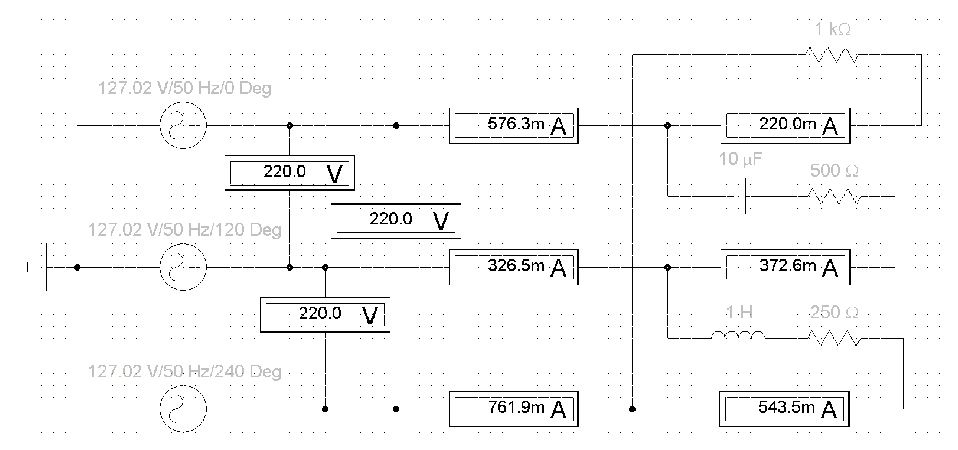
\includegraphics[scale=0.96]{simulacion/practica4.2.eps}
\caption{Simulación del circuito con secuencia positiva.}
\label{simulacion1}
\end{figure}

\begin{figure}[!h]
\centering
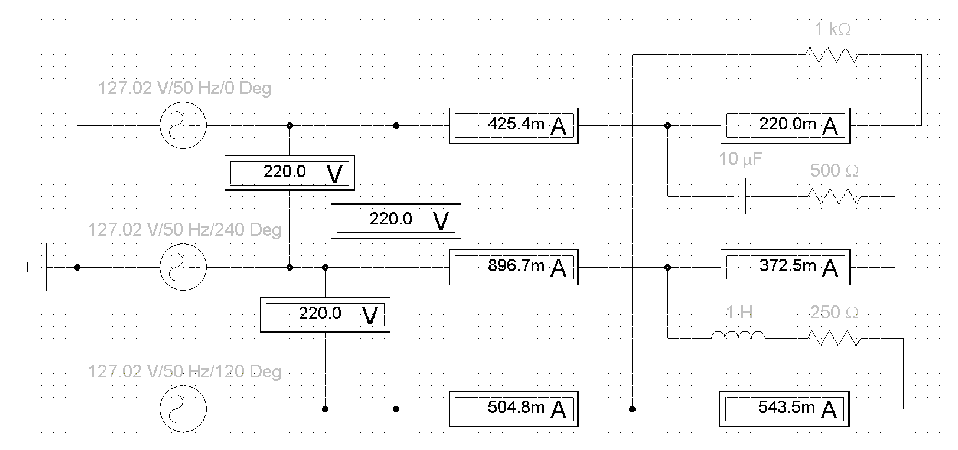
\includegraphics[scale=0.96]{simulacion/practica4.1.eps}
\caption{Simulación del circuito con secuencia negativa.}
\label{simulacion2}
\end{figure}

\section{Tablas y mediciones}
En las tablas siguientes, se presentan los resultados obtenidos con las
mediciones realizadas en laboratorio.

\begin{center}
    \begin{tabular}{|c||c|c|c||c|c|c|}
    \hline
    \textbf{Secuencia} &
    $U_{L_1L_2}[\text{V}]$ & $U_{L_2L_3}[\text{V}]$ & $U_{L_3L_1}[\text{V}]$ &
    $I_{L_1}[\text{A}]$ & $I_{L_2}[\text{A}]$ & $I_{L_3}[\text{A}]$
    \tabularnewline \hline \hline
    $(+)$ & $228$ & $228$ & $227$ & $0.58$ & $0.71$ & $0.33$
    \tabularnewline \hline
    $(-)$ & $228$ & $227$ & $228$ & $0.43$ & $0.48$ & $0.90$
    \tabularnewline \hline
    \end{tabular}
\end{center}

\begin{center}
    \begin{tabular}{|c||c|c|c|}
    \hline
    \textbf{Secuencia} &
    $I_{Z_1}[\text{A}]$ & $I_{Z_2}[\text{A}]$ & $I_{Z_3}[\text{A}]$
    \tabularnewline \hline \hline
    $(+)$ & $0.21$ & $0.51$ & $0.37$
    \tabularnewline \hline
    $(-)$ & $0.21$ & $0.51$ & $0.37$
    \tabularnewline \hline
    \end{tabular}
\end{center}

\section{Cuestionario}

\begin{enumerate}

\item \textbf{Verificar que las corrientes de linea fasoriales suman cero con
los valores teóricos.}

Para la secuencia positiva:
\begin{equation*}
    \begin{split}
        I_{L_1}+I_{L_2}+I_{L_3}\\
        0.58\phase{-17.34^{\circ}}[\text{A}]+
        0.77\phase{-173.92^{\circ}}[\text{A}]+
        0.33\phase{49.89^{\circ}}[\text{A}]\\
        0\phase{0^{\circ}}[\text{A}]\\
    \end{split}
\end{equation*}

Para la secuencia negativa:
\begin{equation*}
    \begin{split}
        I_{L_1}+I_{L_2}+I_{L_3}\\
        0.42\phase{61.19^{\circ}}[\text{A}]+
        0.51\phase{92.17^{\circ}}[\text{A}]+
        0.90\phase{-101.84^{\circ}}[\text{A}]\\
        0\phase{0^{\circ}}[\text{A}]\\
    \end{split}
\end{equation*}

\item \textbf{Comparar los valores obtenidos en secuencia positiva y negativa.
¿Qué corrientes varían y qué corrientes no varían y a qué se debe?}

Las corrientes de fase no varían en magnitud, pero si en fase entre la secuencia
positiva y negativa; mientras que las corrientes de linea varían tanto en
magnitud como en fase.

Este comportamiento se debe al desbalance entre las impedancias conectadas.

\item \textbf{Si la carga conectada en delta la conectamos en estrella,
conectando a $L_1$ la carga resistiva, a $L_2$ la carga $R-L$ y a $L_3$ la carga
$R-C$. ¿Cuál sería el valor de cada corriente de linea?}

\begin{figure}[!h]
\centering
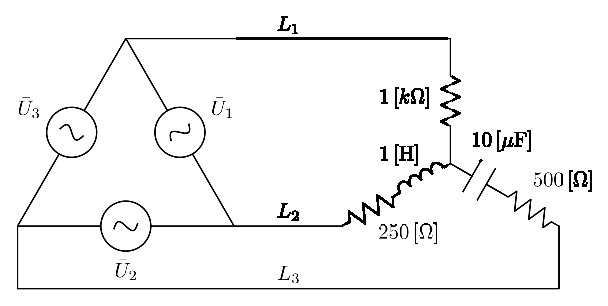
\includegraphics[scale=1.00]{figura2.eps}
\caption{Circuito trifásico desequilibrado delta-estrella.}
\label{circuito2}
\end{figure}

Considerando un circuito trifásico delta-estrella desequilibrado
(\textbf{Figura~\ref{circuito2}}), se hallan las corrientes de linea por medio
de la ley de tensiones de \emph{Kirchhoff}.

Para una secuencia positiva, se tiene:
\begin{equation*}
    \begin{cases}
        -\bar{U}_{L_1L_2}+\bar{I}_a\,Z_1+(\bar{I}_a-\bar{I}_b)\,Z_2=0\\
        -\bar{U}_{L_2L_3}+(\bar{I}_b-\bar{I}_a)\,Z_2+\bar{I}_b\,Z_3=0\\
    \end{cases}
\end{equation*}

\begin{equation*}
    \begin{bmatrix}
        Z_1+Z_2 & -Z_2\\
        -Z_2    & Z_2+Z_3\\
    \end{bmatrix}
    \begin{bmatrix}
        \bar{I}_a \\
        \bar{I}_b \\
    \end{bmatrix}
    =
    \begin{bmatrix}
        \bar{U}_{L_1L_2}\\
        \bar{U}_{L_2L_3}\\
    \end{bmatrix}
\end{equation*}

\begin{equation*}
    \begin{split}
        \bar{I}_a &= \dfrac{\begin{vmatrix}
                        \bar{U}_{L_1L_2} & -Z_2\\
                        \bar{U}_{L_2L_3} & Z_2+Z_3\\
                     \end{vmatrix}}{\begin{vmatrix}
                        Z_1+Z_2 & -Z_2\\
                        -Z_2    & Z_2+Z_3\\
                     \end{vmatrix}}\\
                  &= \dfrac{\bar{U}_{L_1L_2}(Z_2+Z_3)+\bar{U}_{L_2L_3}(Z_2)}
                     {(Z_1+Z_2)(Z_2+Z_3)-(Z_2)^2}\\
                  &= 0.22\phase{-27.44^{\circ}}[\text{A}]\\
    \end{split}
\end{equation*}
\begin{equation*}
    \begin{split}
        \bar{I}_b &= \dfrac{\begin{vmatrix}
                        Z_1+Z_2 & \bar{U}_{L_1L_2}\\
                        -Z_2    & \bar{U}_{L_2L_3}\\
                     \end{vmatrix}}{\begin{vmatrix}
                        Z_1+Z_2 & -Z_2\\
                        -Z_2    & Z_2+Z_3\\
                     \end{vmatrix}}\\
                  &= \dfrac{\bar{U}_{L_2L_3}(Z_1+Z_2)+\bar{U}_{L_1L_2}(Z_2)}
                     {(Z_1+Z_2)(Z_2+Z_3)-(Z_2)^2}\\
                  &= 0.21\phase{-100.65^{\circ}}[\text{A}]\\
    \end{split}
\end{equation*}

Por tanto, las corrientes de linea son:
\begin{equation*}
    \begin{split}
        \bar{I}_1 = \bar{I}_a = 0.22\phase{-27.44^{\circ}}[\text{A}]\\
        \bar{I}_2 = \bar{I}_b-\bar{I}_a = 0.26\phase{-155.59^{\circ}}[\text{A}]\\
        \bar{I}_3 = -\bar{I}_b = 0.21\phase{79.35^{\circ}}[\text{A}]\\
    \end{split}
\end{equation*}

Para una secuencia negativa, se tiene:
\begin{equation*}
    \begin{split}
        \bar{I}_a &= \dfrac{\begin{vmatrix}
                        \bar{U}_{L_1L_2} & -Z_2\\
                        \bar{U}_{L_2L_3} & Z_2+Z_3\\
                     \end{vmatrix}}{\begin{vmatrix}
                        Z_1+Z_2 & -Z_2\\
                        -Z_2    & Z_2+Z_3\\
                     \end{vmatrix}}\\
                  &= \dfrac{\bar{U}_{L_1L_2}(Z_2+Z_3)+\bar{U}_{L_2L_3}(Z_2)}
                     {(Z_1+Z_2)(Z_2+Z_3)-(Z_2)^2}\\
                  &= 0.08\phase{4.60^{\circ}}[\text{A}]\\
    \end{split}
\end{equation*}
\begin{equation*}
    \begin{split}
        \bar{I}_b &= \dfrac{\begin{vmatrix}
                        Z_1+Z_2 & \bar{U}_{L_1L_2}\\
                        -Z_2    & \bar{U}_{L_2L_3}\\
                     \end{vmatrix}}{\begin{vmatrix}
                        Z_1+Z_2 & -Z_2\\
                        -Z_2    & Z_2+Z_3\\
                     \end{vmatrix}}\\
                  &= \dfrac{\bar{U}_{L_2L_3}(Z_1+Z_2)+\bar{U}_{L_1L_2}(Z_2)}
                     {(Z_1+Z_2)(Z_2+Z_3)-(Z_2)^2}\\
                  &= 0.31\phase{113.26^{\circ}}[\text{A}]\\
    \end{split}
\end{equation*}

Por tanto, las corrientes de linea son:
\begin{equation*}
    \begin{split}
        \bar{I}_1 = \bar{I}_a = 0.08\phase{4.60^{\circ}}[\text{A}]\\
        \bar{I}_2 = \bar{I}_b-\bar{I}_a = 0.35\phase{125.87^{\circ}}[\text{A}]\\
        \bar{I}_3 = -\bar{I}_b = 0.31\phase{-66.74^{\circ}}[\text{A}]\\
    \end{split}
\end{equation*}

\end{enumerate}

\section{Conclusiones y Recomendaciones}
Se calcularon, simularon y demostraron experimentalmente la conexión de las
impedancias desbalanceadas en delta comprobándose las relaciones halladas en la
teoría de circuitos eléctricos, y corroboradas por las simulaciones realizadas.

Es recomendable al armar los circuitos en laboratorio revisar apropiadamente los
multímetros para la medición de corriente y voltaje, ya que puede ser peligroso
para los equipos cualquier descuido, esto es aun mas delicado en una conexión
tipo delta.

También se pudo observar que la secuencia de una fuente trifásica puede hallarse
por medio de los valores de corriente obtenidos, y pueden ser intercambiadas
(de positivo a negativo y viceversa) por medio del intercambio entre las lineas
$L_2$ y $L_3$.

\end{document}

